%============================================================
%  RCM OPERATIONAL DEEP-DIVE
%  Engineer: Abdulrahman Hamdi — AI Engineer
%  Compile: pdflatex x2
%============================================================
\documentclass[11pt,a4paper]{article}

\usepackage[T1]{fontenc}
\usepackage[utf8]{inputenc}
\usepackage{mathptmx}
\usepackage[scaled=0.92]{helvet}
\usepackage{courier}
\usepackage{microtype}
\usepackage[top=2.5cm,bottom=2.5cm,left=2.5cm,right=2.5cm,headheight=16pt]{geometry}
\usepackage{xcolor}
\usepackage{graphicx}
\usepackage{amsmath}
\usepackage{booktabs}
\usepackage{array}
\usepackage{colortbl}
\usepackage{multicol}
\usepackage{enumitem}
\usepackage{fancyhdr}
\usepackage{titlesec}
\usepackage{tcolorbox}
\usepackage{tikz}
\usepackage{pgfplots}
\usepackage{mdframed}
\usepackage{hyperref}
\usepackage{tabularx}

\usetikzlibrary{shapes.geometric,arrows.meta,positioning,fit,calc,shadows,backgrounds}
\tcbuselibrary{skins,breakable}
\pgfplotsset{compat=1.18}

%-----------------------------------------------------------
% COLOURS
%-----------------------------------------------------------
\definecolor{PrimaryBlue}{HTML}{1A3C5E}
\definecolor{AccentTeal}{HTML}{0D7C8C}
\definecolor{AccentGold}{HTML}{C8962A}
\definecolor{LightBg}{HTML}{F4F7FA}
\definecolor{MidGray}{HTML}{6B7B8D}
\definecolor{DangerRed}{HTML}{C0392B}
\definecolor{SuccessGreen}{HTML}{1E8449}
\definecolor{WarningAmber}{HTML}{D4850A}
\definecolor{SoftBlue}{HTML}{D6E4F0}
\definecolor{SoftTeal}{HTML}{D0EEF2}
\definecolor{SoftGold}{HTML}{FAF0DC}
\definecolor{SoftRed}{HTML}{FADBD8}
\definecolor{SoftGreen}{HTML}{D5F5E3}
\definecolor{TableHead}{HTML}{1A3C5E}
\definecolor{TableAlt}{HTML}{EAF2FA}
\definecolor{RuleColor}{HTML}{B0C4D8}

%-----------------------------------------------------------
% HYPERREF
%-----------------------------------------------------------
\hypersetup{colorlinks=true,linkcolor=PrimaryBlue,urlcolor=AccentTeal,
  pdftitle={RCM Operational Deep-Dive --- Authorization \& Billing},bookmarksnumbered=true}

%-----------------------------------------------------------
% HEADER / FOOTER
%-----------------------------------------------------------
\pagestyle{fancy}\fancyhf{}
\fancyhead[L]{\color{MidGray}\small\textit{RCM \& Insurance Authorization Workflow --- AI Department}}
\fancyhead[R]{\color{MidGray}\small\textit{Eng.\ Abdulrahman Hamdi}}
\fancyfoot[C]{\color{MidGray}\thepage}
\renewcommand{\headrulewidth}{0.4pt}
\renewcommand{\headrule}{\hbox to\headwidth{\color{RuleColor}\leaders\hrule height\headrulewidth\hfill}}

%-----------------------------------------------------------
% SECTION STYLING
%-----------------------------------------------------------
\titleformat{\section}{\color{PrimaryBlue}\Large\bfseries}
  {\colorbox{PrimaryBlue}{\color{white}\ \thesection\ }}{0.8em}{}
  [\vspace{-0.2em}\color{RuleColor}\rule{\linewidth}{1.5pt}\vspace{0.3em}]
\titleformat{\subsection}{\color{AccentTeal}\large\bfseries}
  {\color{AccentTeal}\thesubsection}{0.6em}{}
  [\vspace{-0.3em}\color{RuleColor}\rule{\linewidth}{0.6pt}]
\titleformat{\subsubsection}{\color{PrimaryBlue}\normalsize\bfseries}
  {\color{AccentGold}\thesubsubsection}{0.5em}{}
\titlespacing*{\section}{0pt}{1.6em}{0.8em}
\titlespacing*{\subsection}{0pt}{1.2em}{0.5em}
\titlespacing*{\subsubsection}{0pt}{0.9em}{0.3em}

%-----------------------------------------------------------
% LISTS
%-----------------------------------------------------------
\setlist[itemize,1]{label={\color{AccentTeal}\textbullet},leftmargin=1.5em,itemsep=0.25em,topsep=0.3em}
\setlist[itemize,2]{label={\color{AccentGold}\small$\blacktriangleright$},leftmargin=1.5em,itemsep=0.15em}
\setlist[enumerate,1]{label={\color{PrimaryBlue}\bfseries\arabic*.},leftmargin=1.8em,itemsep=0.25em}

%-----------------------------------------------------------
% TCOLORBOX STYLES
%-----------------------------------------------------------
\tcbset{
  infobox/.style={enhanced,breakable,colback=SoftBlue,colframe=PrimaryBlue,
    boxrule=1.2pt,arc=4pt,left=8pt,right=8pt,top=6pt,bottom=6pt,
    fonttitle=\bfseries\color{white},
    attach boxed title to top left={yshift=-2mm,xshift=6mm},
    boxed title style={colback=PrimaryBlue,arc=3pt,boxrule=0pt}},
  warnbox/.style={enhanced,breakable,colback=SoftGold,colframe=WarningAmber,
    boxrule=1.2pt,arc=4pt,left=8pt,right=8pt,top=6pt,bottom=6pt,
    fonttitle=\bfseries\color{white},
    attach boxed title to top left={yshift=-2mm,xshift=6mm},
    boxed title style={colback=WarningAmber,arc=3pt,boxrule=0pt}},
  dangerbox/.style={enhanced,breakable,colback=SoftRed,colframe=DangerRed,
    boxrule=1.2pt,arc=4pt,left=8pt,right=8pt,top=6pt,bottom=6pt,
    fonttitle=\bfseries\color{white},
    attach boxed title to top left={yshift=-2mm,xshift=6mm},
    boxed title style={colback=DangerRed,arc=3pt,boxrule=0pt}},
  successbox/.style={enhanced,breakable,colback=SoftGreen,colframe=SuccessGreen,
    boxrule=1.2pt,arc=4pt,left=8pt,right=8pt,top=6pt,bottom=6pt,
    fonttitle=\bfseries\color{white},
    attach boxed title to top left={yshift=-2mm,xshift=6mm},
    boxed title style={colback=SuccessGreen,arc=3pt,boxrule=0pt}},
  statbox/.style={enhanced,colback=LightBg,colframe=AccentGold,
    boxrule=2pt,arc=6pt,left=10pt,right=10pt,top=8pt,bottom=8pt},
  rulebox/.style={enhanced,breakable,colback=LightBg,colframe=PrimaryBlue,
    boxrule=0.8pt,arc=3pt,left=7pt,right=7pt,top=6pt,bottom=6pt,
    borderline west={3pt}{0pt}{AccentTeal}},
  metricbox/.style={enhanced,colback=white,colframe=AccentTeal,
    boxrule=1.4pt,arc=6pt,left=8pt,right=8pt,top=8pt,bottom=8pt,
    drop shadow}
}

%-----------------------------------------------------------
% TIKZ BASE STYLES
%-----------------------------------------------------------
\tikzset{
  FB/.style={rectangle,rounded corners=3pt,
             minimum width=2.6cm,minimum height=0.85cm,
             text centered,align=center,draw,thick,
             font=\footnotesize\bfseries},
  DM/.style={diamond,aspect=2.0,
             minimum width=2.4cm,minimum height=0.75cm,
             text centered,align=center,draw,thick,
             font=\footnotesize\bfseries},
  arr/.style={-{Stealth[length=4.5pt]},thick},
  nB/.style={FB,fill=SoftBlue, draw=PrimaryBlue,text=PrimaryBlue},
  nT/.style={FB,fill=SoftTeal, draw=AccentTeal, text=AccentTeal},
  nG/.style={FB,fill=SoftGold, draw=AccentGold, text=AccentGold},
  nR/.style={FB,fill=SoftRed,  draw=DangerRed,  text=DangerRed},
  nV/.style={FB,fill=SoftGreen,draw=SuccessGreen,text=SuccessGreen},
  dB/.style={DM,fill=SoftBlue, draw=PrimaryBlue,text=PrimaryBlue},
  dT/.style={DM,fill=SoftTeal, draw=AccentTeal, text=AccentTeal},
  dG/.style={DM,fill=SoftGold, draw=AccentGold, text=AccentGold},
  LY/.style={font=\scriptsize\bfseries\color{SuccessGreen},midway,auto},
  LN/.style={font=\scriptsize\bfseries\color{DangerRed},midway,auto}
}

%-----------------------------------------------------------
% HELPERS
%-----------------------------------------------------------
\newcolumntype{L}[1]{>{\raggedright\arraybackslash}p{#1}}
\newcolumntype{C}[1]{>{\centering\arraybackslash}p{#1}}

%============================================================
\begin{document}
%============================================================

%------------------------------------------------------------
% COVER PAGE
%------------------------------------------------------------
\begin{titlepage}
\pagecolor{PrimaryBlue}\color{white}
\vspace*{0.8cm}
\begin{center}
  \textcolor{AccentGold}{\rule{0.88\linewidth}{2pt}}\\[0.3em]
  \textcolor{AccentGold}{\rule{0.88\linewidth}{0.5pt}}\\[1.6cm]

  {\fontsize{32}{40}\selectfont\bfseries Operational Deep-Dive}\\[0.3em]
  {\fontsize{22}{30}\selectfont\bfseries Revenue Cycle Management}\\[0.2em]
  {\fontsize{20}{28}\selectfont\bfseries \& Insurance Authorization Workflow}\\[1.0em]

  \textcolor{AccentGold}{\rule{0.5\linewidth}{0.8pt}}\\[0.8em]
  {\color{SoftBlue}\small
    Patient Filtering \textbullet{} Authorization \textbullet{}
    Billing Pipeline \textbullet{} Claim Submission \textbullet{} Quality Control}\\[2.4cm]

  \begin{tabular}{@{}ll@{}}
    \textcolor{AccentGold}{\bfseries Department:} & Revenue Cycle Management \\[0.3em]
    \textcolor{AccentGold}{\bfseries Prepared by:} & Eng.\ Abdulrahman Hamdi --- AI Engineer \\[0.3em]
    \textcolor{AccentGold}{\bfseries Version:} & 1.0 \\[0.3em]
    \textcolor{AccentGold}{\bfseries Year:} & 2026 \\
  \end{tabular}

  \vfill
  \textcolor{AccentGold}{\rule{0.88\linewidth}{0.5pt}}\\[0.3em]
  \textcolor{AccentGold}{\rule{0.88\linewidth}{2pt}}
\end{center}
\end{titlepage}
\nopagecolor\color{black}

%------------------------------------------------------------
% TABLE OF CONTENTS
%------------------------------------------------------------
\newpage
\tableofcontents
\newpage

%============================================================
\section{Executive Introduction: The Strategic Role of Authorization and Billing Systems}
%============================================================

In the high-stakes environment of healthcare Revenue Cycle Management (RCM), the synchronization of insurance authorization, patient filtering, and billing submission is not merely an administrative task; it is a strategic imperative. A seamless integration ensures that clinical services are rendered only when financial coverage is secured, directly protecting the clinic's bottom line and minimizing the risk of unpaid claims. When authorization data flows accurately from the point of intake to final submission, it reduces administrative friction and enhances the overall financial health and operational efficiency of the clinic.

The objective of this document is to provide a comprehensive blueprint of the patient journey within our RCM ecosystem. By synthesizing operational meeting notes, we map the progression from the initial intake to final claim submission. We begin this journey at the foundational stage of the process: Patient Filtering.

\vspace{0.5em}
\begin{center}
\textbf{\color{PrimaryBlue}End-to-End RCM Journey --- From Intake to Claim Submission}\\[0.6em]
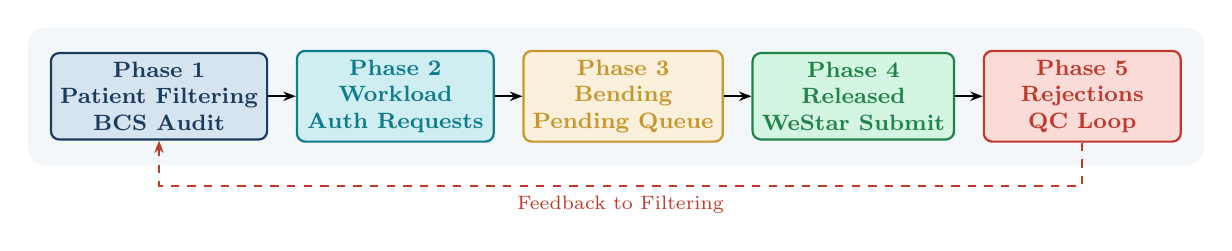
\begin{tikzpicture}[node distance=0.45cm and 0.35cm,every node/.style={align=center,font=\scriptsize\bfseries}]
  \node[nB,minimum width=2.5cm] (filter) {Phase 1\\Patient Filtering\\BCS Audit};
  \node[nT,minimum width=2.5cm,right=0.35cm of filter] (auth) {Phase 2\\Workload\\Auth Requests};
  \node[nG,minimum width=2.5cm,right=0.35cm of auth] (bend) {Phase 3\\Bending\\Pending Queue};
  \node[nV,minimum width=2.5cm,right=0.35cm of bend] (release) {Phase 4\\Released\\WeStar Submit};
  \node[nR,minimum width=2.5cm,right=0.35cm of release] (reject) {Phase 5\\Rejections\\QC Loop};

  \draw[arr](filter)--(auth);
  \draw[arr](auth)--(bend);
  \draw[arr](bend)--(release);
  \draw[arr](release)--(reject);

  \draw[arr,dashed,DangerRed,thick]
    (reject.south)--++(0,-0.55)-|
    node[below,font=\scriptsize\color{DangerRed},pos=0.25]{Feedback to Filtering}
    (filter.south);

  \begin{scope}[on background layer]
    \node[fill=LightBg,rounded corners=6pt,inner sep=8pt,
          fit=(filter)(auth)(bend)(release)(reject)] {};
  \end{scope}
\end{tikzpicture}
\end{center}

\begin{tcolorbox}[statbox]
\begin{center}
  \Large\bfseries\color{PrimaryBlue}Strategic Objective\\[0.4em]
  \normalsize
  Map the complete RCM operating model from patient filtering and authorization
  through billing release, clearinghouse submission, and rejection correction.
  Every control in this document protects one of four outcomes:
\end{center}
\vspace{0.3em}
\begin{center}
\begin{tabularx}{0.96\linewidth}{C{3.1cm} C{3.1cm} C{3.1cm} C{3.1cm}}
  \textcolor{PrimaryBlue}{\bfseries Coverage} &
  \textcolor{AccentTeal}{\bfseries Authorization} &
  \textcolor{AccentGold}{\bfseries Billing Accuracy} &
  \textcolor{DangerRed}{\bfseries Cash Flow} \\
  Valid insurance on file &
  Pre-approval secured &
  Clean claim release &
  Denials prevented \\
\end{tabularx}
\end{center}
\end{tcolorbox}


%============================================================
\section{The Patient Filtering and ``Can Be Seen'' (BCS) Methodology}
%============================================================

The filtering phase serves as the primary gateway for risk mitigation and revenue protection. By auditing patient records before they are seen by a provider, the RCM team ensures that every visit is backed by a valid authorization or an active insurance policy, thereby preventing revenue leakage at the source.

\subsection{The ``Can Be Seen'' (BCS) Logic}

The RCM team utilizes a binary logic to determine patient eligibility for daily appointments:

\begin{itemize}
  \item \textbf{BCS --- Yes:} The patient meets all criteria, including active coverage and a valid authorization that covers the specific date of service.
  \item \textbf{BCS --- No:} The patient is restricted from being seen. Common reasons include:
  \begin{itemize}
    \item \textbf{Expiry:} The existing authorization has passed its end date.
    \item \textbf{New Request Needed:} The patient has exhausted their allotted visits (e.g., 5 out of 5 visits used).
    \item \textbf{Pending Authorization:} A request has been submitted to the insurance provider, but no approval has been received yet.
  \end{itemize}
\end{itemize}

\vspace{0.4em}
\begin{center}
\textbf{\color{AccentTeal}Diagram A --- BCS Decision Tree}\\[0.5em]
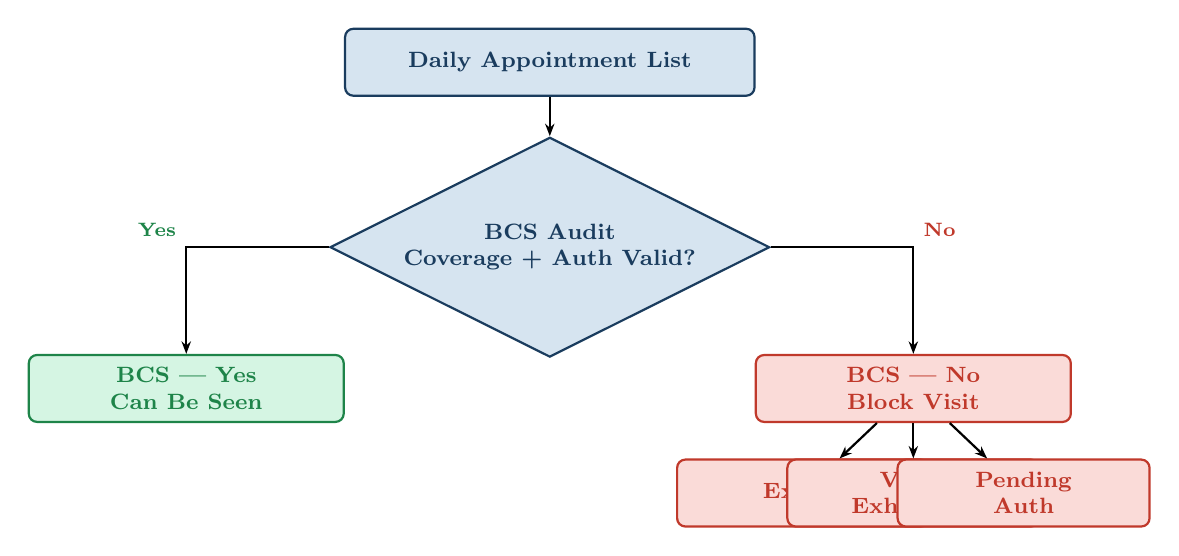
\begin{tikzpicture}[node distance=0.5cm,every node/.style={align=center}]
  \node[nB,minimum width=5.2cm] (list) {Daily Appointment List};
  \node[dB,minimum width=4.8cm,below=0.5cm of list] (audit) {BCS Audit\\Coverage + Auth Valid?};
  \node[nV,minimum width=4.0cm,below left=0.65cm and 1.2cm of audit] (yes) {BCS --- Yes\\Can Be Seen};
  \node[nR,minimum width=4.0cm,below right=0.65cm and 1.2cm of audit] (no) {BCS --- No\\Block Visit};
  \node[nR,minimum width=3.2cm,below=0.45cm of no,xshift=-1.4cm] (exp) {Expiry};
  \node[nR,minimum width=3.2cm,below=0.45cm of no] (exh) {Visits\\Exhausted};
  \node[nR,minimum width=3.2cm,below=0.45cm of no,xshift=1.4cm] (pend) {Pending\\Auth};

  \draw[arr](list)--(audit);
  \draw[arr](audit.west)-| node[LY,above left]{Yes} (yes.north);
  \draw[arr](audit.east)-| node[LN,above right]{No} (no.north);
  \draw[arr](no)--(exp);
  \draw[arr](no)--(exh);
  \draw[arr](no)--(pend);
\end{tikzpicture}
\end{center}

\subsection{Initial Exams vs.\ Follow-up Visits}

The workflow distinguishes between patient types to manage workload efficiency. Initial visits (Exams) are typically processed through the ``Workload'' department, as these require the first-time establishment of authorization. Follow-up visits are audited via the ``Filtering'' sheet to ensure ongoing compliance. While initial visits for certain plans (like Workers' Compensation) are often approved for a single encounter to allow for the creation of a Plan of Care (POC), subsequent visits must be strictly audited.

\vspace{0.4em}
\begin{center}
\textbf{\color{AccentTeal}Diagram B --- Exam vs.\ Follow-up Routing}\\[0.5em]
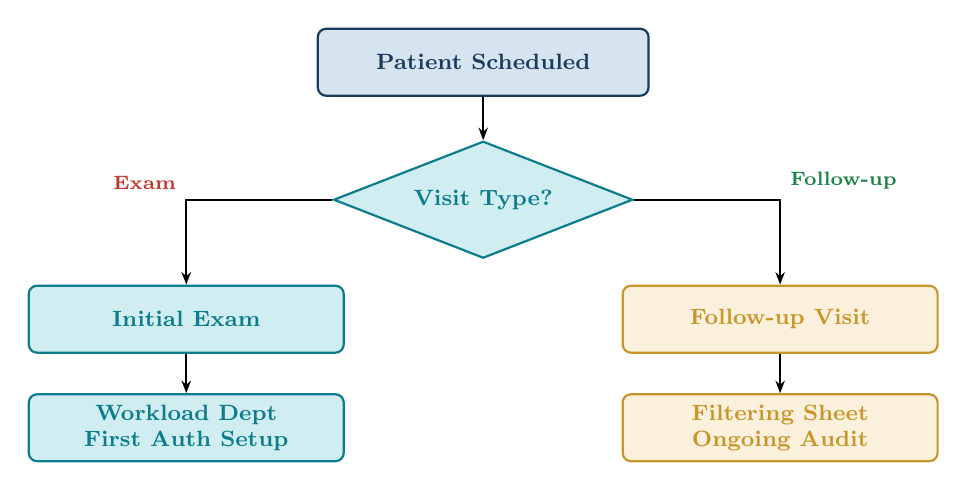
\begin{tikzpicture}[node distance=0.5cm and 1.0cm,every node/.style={align=center}]
  \node[nB,minimum width=4.2cm] (patient) {Patient Scheduled};
  \node[dT,minimum width=3.8cm,below=0.55cm of patient] (type) {Visit Type?};

  \node[nT,minimum width=4.0cm,below left=0.7cm and 0.8cm of type] (exam) {Initial Exam};
  \node[nG,minimum width=4.0cm,below right=0.7cm and 0.8cm of type] (follow) {Follow-up Visit};

  \node[nT,minimum width=4.0cm,below=0.5cm of exam] (workload) {Workload Dept\\First Auth Setup};
  \node[nG,minimum width=4.0cm,below=0.5cm of follow] (filtering) {Filtering Sheet\\Ongoing Audit};

  \draw[arr](patient)--(type);
  \draw[arr](type.west)-| node[LN,above left]{Exam} (exam.north);
  \draw[arr](type.east)-| node[LY,above right]{Follow-up} (follow.north);
  \draw[arr](exam)--(workload);
  \draw[arr](follow)--(filtering);
\end{tikzpicture}
\end{center}

\subsection{Knowledge Management and Communication}

The effectiveness of the filtering process relies on a blend of ``experience-based'' knowledge and real-time data updates. Rather than relying solely on static manuals, the team utilizes internal ``Cluster Chats'' to circulate insurance updates. Experienced specialists maintain personalized tracking sheets to ensure data accuracy across the team, specifically regarding shifting portal requirements.

\begin{tcolorbox}[rulebox,title={Knowledge Management Principle}]
Filtering accuracy depends on live payer intelligence. Cluster Chats and specialist tracking sheets are not optional supplements --- they are operational controls that keep BCS decisions aligned with current portal behavior.
\end{tcolorbox}


%============================================================
\section{Authorization Management and Workload Execution}
%============================================================

The Workload department is responsible for the technical execution of authorization requests. This team secures pre-approvals before clinical services are rendered, navigating a complex landscape of payer-specific portals and manual submission methods.

\subsection{Insurance Behavior and Action Requirements}

Different insurance carriers exhibit unique behaviors regarding how they process and approve visits. The following table outlines specific behaviors identified in the operational workflow:

\begin{tcolorbox}[infobox,title={Insurance Behavior Matrix}]
\small
\begin{tabularx}{\linewidth}{L{2.4cm} X L{3.4cm}}
  \rowcolor{TableHead}
  \color{white}\textbf{Insurance Type} & \color{white}\textbf{Request Behavior} & \color{white}\textbf{Action Required} \\
  \textbf{MetroPlus}
    & Unreliable portal; requires faxed requests.
    & Fax submission; call to verify status after 4 days. \\
  \rowcolor{TableAlt}
  \textbf{Integra}
    & Allows 3 visits within a 3-week window before a hard stop.
    & Monitor visit count; place on ``Hold'' after 3rd visit until auth is secured. \\
  \textbf{Medicare}
    & Federal plan; IDs typically start with an `R' prefix.
    & ``Fake Auths'' are not used; verify benefits and monitor the \$2{,}000 cap. \\
  \rowcolor{TableAlt}
  \textbf{HealthFirst}
    & Portal-specific requirements; requires alignment of diagnosis codes.
    & Use the HealthFirst portal for real-time status checks and approvals. \\
  \textbf{Workers' Comp}
    & High-risk; rarely allows back-dated authorizations.
    & Strict monitoring; immediate ``Hard Stop'' if authorization is not on file. \\
\end{tabularx}
\end{tcolorbox}

\subsection{The ``Bending'' (Pending) Workflow}

Within the billing system, ``Bending'' refers to the Pending Charges queue. This is a specific location in WebPT Billing where charges are held before they are ``Released.'' The ``So What?'' layer of this status is determined by the specific insurer:

\begin{itemize}
  \item \textbf{Commercial/Risk-Tolerant:} Certain insurers (like Integra) allow a 3-week or 3-visit grace period while authorization is ``Bending.''
  \item \textbf{High-Volatility:} Workers' Compensation and No-Fault require immediate holds. If the charge is in the Bending queue without a confirmed authorization, the patient cannot be seen because these payers rarely back-date approvals.
\end{itemize}

\vspace{0.4em}
\begin{center}
\textbf{\color{AccentTeal}Diagram C --- Bending Workflow by Payer Risk}\\[0.5em]
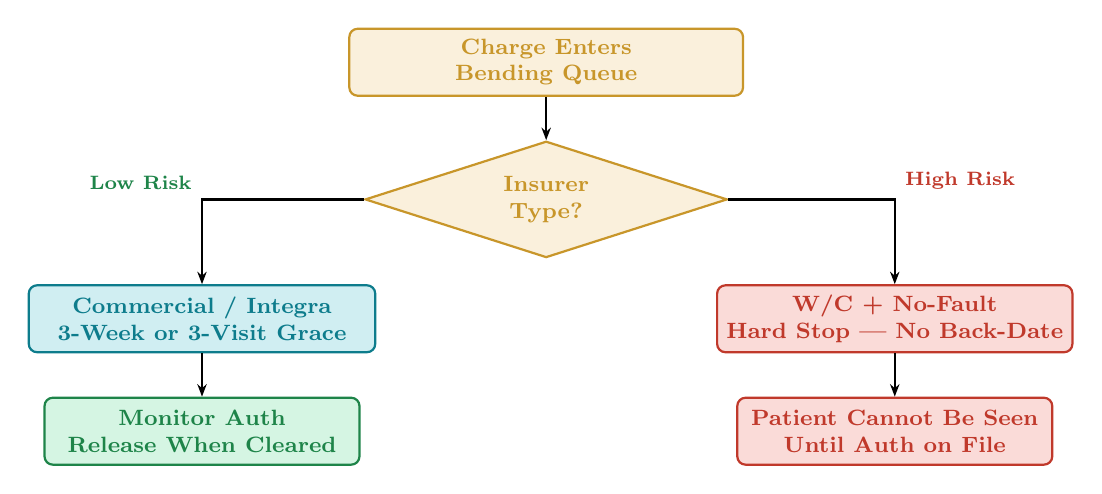
\begin{tikzpicture}[node distance=0.5cm,every node/.style={align=center}]
  \node[nG,minimum width=5.0cm] (enter) {Charge Enters\\Bending Queue};
  \node[dG,minimum width=4.6cm,below=0.55cm of enter] (ins) {Insurer\\Type?};
  \node[nT,minimum width=4.4cm,below left=0.7cm and 1.0cm of ins] (comm) {Commercial / Integra\\3-Week or 3-Visit Grace};
  \node[nR,minimum width=4.4cm,below right=0.7cm and 1.0cm of ins] (hv) {W/C + No-Fault\\Hard Stop --- No Back-Date};
  \node[nV,minimum width=4.0cm,below=0.55cm of comm] (wait) {Monitor Auth\\Release When Cleared};
  \node[nR,minimum width=4.0cm,below=0.55cm of hv] (stop) {Patient Cannot Be Seen\\Until Auth on File};

  \draw[arr](enter)--(ins);
  \draw[arr](ins.west)-| node[LY,above left]{Low Risk} (comm.north);
  \draw[arr](ins.east)-| node[LN,above right]{High Risk} (hv.north);
  \draw[arr](comm)--(wait);
  \draw[arr](hv)--(stop);
\end{tikzpicture}
\end{center}

\begin{tcolorbox}[warnbox,title={Integra 3-Visit Hold Rule}]
After the 3rd visit within a 3-week window, the patient must be placed on Hold until a new authorization is secured. Do not allow additional visits during this gap --- Integra will hard-stop billing.
\end{tcolorbox}


%============================================================
\section{Systems Integration: WebPT to WeStar Data Synchronization}
%============================================================

The technical ecosystem relies on the seamless transfer of data between the WebPT EMR (clinical notes), WebPT Billing (claim preparation), and the WeStar Clearinghouse (claim transmission).

\subsection{The Billing Exception Workflow}

Data often fails to sync correctly between the EMR and the billing platform, resulting in ``Billing Exceptions.'' These must be cleared before a claim can proceed. Common synchronization failures include:

\begin{tcolorbox}[infobox,title={Common Billing Exceptions}]
\begin{enumerate}
  \item \textbf{Address Mismatches:} Discrepancies between the patient's address in the clinical file versus the billing record.
  \item \textbf{Missing Provider Credentials:} Providers added to the EMR but not yet credentialed or linked within the WebPT Billing platform.
  \item \textbf{Case ID Errors:} Clinical notes being closed under the wrong ``Case,'' preventing the system from identifying the correct payer.
\end{enumerate}
\end{tcolorbox}

\vspace{0.4em}
\begin{center}
\textbf{\color{AccentTeal}Diagram D --- System Architecture: WebPT to WeStar}\\[0.5em]
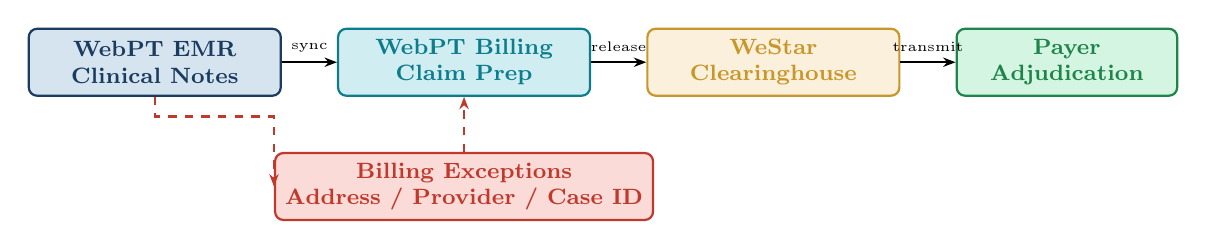
\begin{tikzpicture}[node distance=0.5cm and 0.6cm,every node/.style={align=center,font=\scriptsize\bfseries}]
  \node[nB,minimum width=3.2cm] (emr) {WebPT EMR\\Clinical Notes};
  \node[nT,minimum width=3.2cm,right=0.7cm of emr] (bill) {WebPT Billing\\Claim Prep};
  \node[nG,minimum width=3.2cm,right=0.7cm of bill] (westar) {WeStar\\Clearinghouse};
  \node[nV,minimum width=2.8cm,right=0.7cm of westar] (payer) {Payer\\Adjudication};

  \draw[arr](emr)--node[above,font=\tiny]{sync}(bill);
  \draw[arr](bill)--node[above,font=\tiny]{release}(westar);
  \draw[arr](westar)--node[above,font=\tiny]{transmit}(payer);

  \node[nR,minimum width=4.8cm,below=0.7cm of bill] (exc) {Billing Exceptions\\Address / Provider / Case ID};
  \draw[arr,DangerRed,dashed](emr.south)--++(0,-0.25)-|(exc.west);
  \draw[arr,DangerRed,dashed](exc.north)--(bill.south);
\end{tikzpicture}
\end{center}

\subsection{The ``Lumbar'' (LMR) Case Study: Diagnostic Alignment}

Operational efficiency requires strict alignment between Case IDs and Diagnosis codes. A common error involves the ``Lumbar'' (shorthand: LMR) case type. If a clinician opens a case named ``Lumbar'' for a back injury but the billing claim includes CPT codes or diagnosis codes for a different body part (e.g., Knee), the claim will be rejected. Case IDs must accurately reflect the clinical Plan of Care to ensure a clean ``Release'' of the charge.

\begin{tcolorbox}[dangerbox,title={Diagram F --- LMR Case Alignment: Wrong vs.\ Right}]
\begin{tabularx}{\linewidth}{@{}X X@{}}
  \textcolor{DangerRed}{\bfseries Wrong --- Rejection Risk} &
  \textcolor{SuccessGreen}{\bfseries Right --- Clean Release} \\[0.4em]
  Case ID = Lumbar (Back) &
  Case ID = Lumbar (Back) \\
  CPT / Dx = Knee codes &
  CPT / Dx = Lumbar / Back codes \\
  \textit{Result: Claim rejected at clearinghouse} &
  \textit{Result: Charge released and transmitted} \\
\end{tabularx}
\end{tcolorbox}

\subsection{The Release Mechanism}

Charges move through a structured pipeline:

\begin{itemize}
  \item \textbf{Bending (Pending):} The queue where charges wait for authorization or audit.
  \item \textbf{Released:} Once audited for accuracy (provider, location, Case ID, and CPT codes), charges are ``Released'' from WebPT Billing.
  \item \textbf{Clearinghouse:} The charges arrive at WeStar for final scrubbing and transmission to the payer.
\end{itemize}

\vspace{0.4em}
\begin{center}
\textbf{\color{AccentTeal}Diagram E --- Release Pipeline}\\[0.5em]

\begin{tikzpicture}[node distance=0.4cm and 0.3cm,every node/.style={align=center,font=\scriptsize\bfseries}]
  \node[nG,minimum width=2.4cm] (bend) {Bending\\Pending};
  \node[nB,minimum width=2.6cm,right=0.35cm of bend] (audit) {Audit\\Provider / Location\\Case ID / CPT};
  \node[nV,minimum width=2.4cm,right=0.35cm of audit] (rel) {Released\\WebPT Billing};
  \node[nT,minimum width=2.4cm,right=0.35cm of rel] (scrub) {WeStar\\Scrub};
  \node[nB,minimum width=2.4cm,right=0.35cm of scrub] (tx) {Payer\\Transmission};

  \draw[arr](bend)--(audit);
  \draw[arr](audit)--(rel);
  \draw[arr](rel)--(scrub);
  \draw[arr](scrub)--(tx);
\end{tikzpicture}
\end{center}


%============================================================
\section{Specialized Billing Streams: Medicare, Workers' Comp, and No-Fault}
%============================================================

Specialized insurance categories require an ``Audit-First'' submission approach due to unique regulatory requirements and high-risk hold criteria.

\subsection{Medicare and the ``Kx Modifier''}

Medicare billing is governed by an annual financial cap (approximately \$2{,}000). To manage this:

\begin{enumerate}
  \item \textbf{Verify Total Spent:} Specialists must pull a Benefit Report or check the Medicare portal to view the ``Total'' amount the patient has spent toward their cap (e.g., \$294 used).
  \item \textbf{Threshold Check:} Once the \$2{,}000 threshold is met, the specialist must manually append the ``Kx Modifier'' to the claim to signal medical necessity.
  \item \textbf{Audit Requirement:} No Medicare claim should be ``Released'' without a prior check of the portal to calculate the remaining balance.
\end{enumerate}

\vspace{0.3em}
\begin{center}
\textbf{\color{AccentTeal}Medicare Cap Usage Chart --- Example Patient}\\[0.4em]
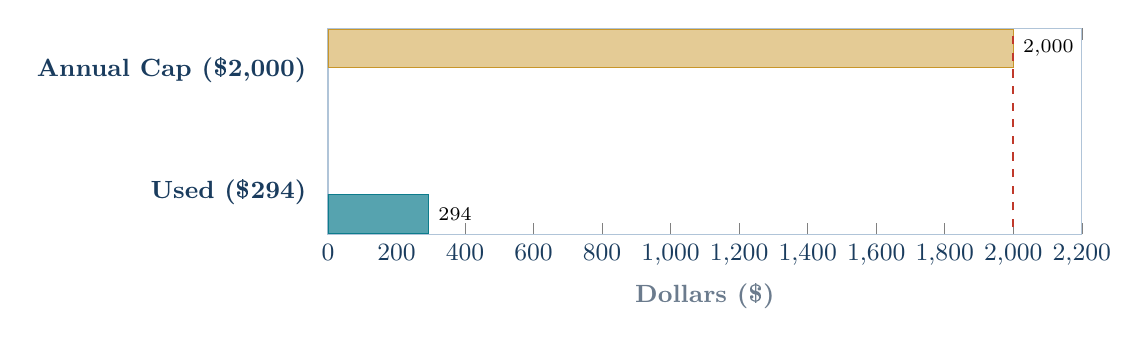
\begin{tikzpicture}
\begin{axis}[
  width=0.92\linewidth,
  height=4.2cm,
  xbar,
  xmin=0, xmax=2200,
  ytick={1,2},
  yticklabels={Used (\$294),Annual Cap (\$2{,}000)},
  ytick style={draw=none},
  axis line style={draw=RuleColor},
  tick label style={font=\small\bfseries,color=PrimaryBlue},
  xlabel={Dollars (\$)},
  xlabel style={font=\small\bfseries,color=MidGray},
  bar width=14pt,
  enlarge y limits=0.35,
  nodes near coords,
  nodes near coords align={horizontal},
  every node near coord/.append style={font=\scriptsize\bfseries},
  legend style={at={(0.98,1.02)},anchor=north east,font=\scriptsize}
]
  \addplot[fill=AccentTeal!70,draw=AccentTeal] coordinates {(294,1)};
  \addplot[fill=AccentGold!50,draw=AccentGold] coordinates {(2000,2)};
  \draw[DangerRed,thick,dashed] (axis cs:2000,0.3) -- (axis cs:2000,2.7)
    node[above,font=\scriptsize\bfseries\color{DangerRed}] {Kx Modifier Required};
\end{axis}
\end{tikzpicture}
\end{center}

\subsection{Workers' Compensation (W/C) and No-Fault (NF)}

These streams are categorized by how the request is initiated:

\begin{itemize}
  \item \textbf{MTG (Medical Treatment Guidelines):} Covers Shoulder, Knee, Back, and Neck. These are provider-driven. The RCM team is dependent on the doctor to submit the Medical Treatment Guideline forms and Plan of Care. A ``Hard Stop'' is often triggered not by portal delays, but by a provider's failure to submit the necessary clinical documentation.
  \item \textbf{Non-MTG:} Covers all other body parts. These are portal-driven and handled directly by the Authorization/Workload team.
\end{itemize}

\subsection{Field Charges (Felt) and Manual Submissions}

Certain plans, such as Medicaid, ``Police,'' or ``Board of Ed'' plans, are categorized as ``Field Charges'' (Felt) because they do not support automatic routing via the clearinghouse.

\begin{itemize}
  \item \textbf{Manual Entry:} These require manual entry into the payer's specific portal or submission via fax.
  \item \textbf{Batching Logic:} These charges are often held until a full Plan of Care (POC) cycle (e.g., 12 visits) is completed. This ensures the manual submission matches the authorized volume for lump-sum payment.
\end{itemize}

\vspace{0.4em}
\begin{center}
\textbf{\color{AccentTeal}Diagram G --- Specialized Billing Streams}\\[0.5em]
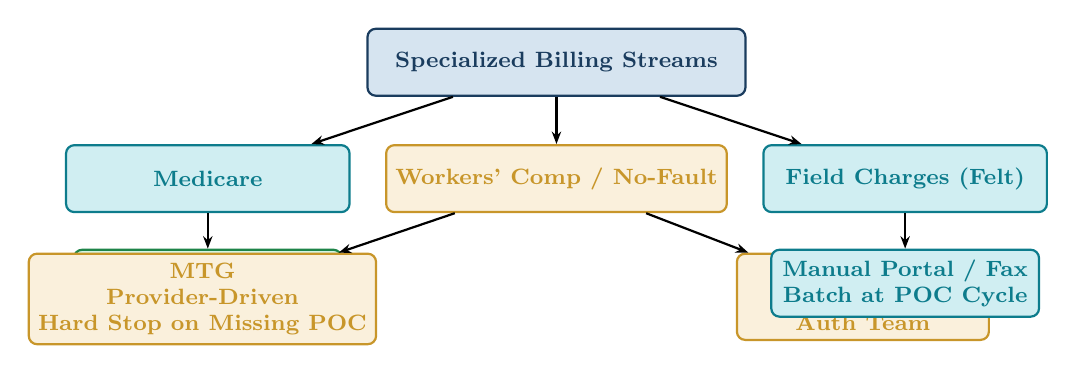
\begin{tikzpicture}[node distance=0.45cm and 0.5cm,every node/.style={align=center,font=\scriptsize\bfseries}]
  \node[nB,minimum width=4.8cm] (root) {Specialized Billing Streams};

  \node[nT,minimum width=3.6cm,below left=0.6cm and 0.2cm of root] (mc) {Medicare};
  \node[nG,minimum width=3.6cm,below=0.6cm of root] (wc) {Workers' Comp / No-Fault};
  \node[nT,minimum width=3.6cm,below right=0.6cm and 0.2cm of root] (felt) {Field Charges (Felt)};

  \node[nV,minimum width=3.4cm,below=0.45cm of mc] (mc2) {Portal Cap Check\\Kx at \$2{,}000};
  \node[nG,minimum width=3.2cm,below left=0.5cm and 0.1cm of wc] (mtg) {MTG\\Provider-Driven\\Hard Stop on Missing POC};
  \node[nG,minimum width=3.2cm,below right=0.5cm and 0.1cm of wc] (nmtg) {Non-MTG\\Portal-Driven\\Auth Team};
  \node[nT,minimum width=3.4cm,below=0.45cm of felt] (felt2) {Manual Portal / Fax\\Batch at POC Cycle};

  \draw[arr](root)--(mc);
  \draw[arr](root)--(wc);
  \draw[arr](root)--(felt);
  \draw[arr](mc)--(mc2);
  \draw[arr](wc)--(mtg);
  \draw[arr](wc)--(nmtg);
  \draw[arr](felt)--(felt2);
\end{tikzpicture}
\end{center}


%============================================================
\section{Quality Control: Rejection Handling and Claim Correction}
%============================================================

The ``Rejection'' phase is the final checkpoint in minimizing Days in Accounts Receivable (AR). Rejections occur when the clearinghouse (WeStar) or the payer identifies an error prior to processing.

\subsection{Common Rejection Categories}

\begin{itemize}
  \item \textbf{Subscriber Name Mismatch:} The patient name on the claim does not exactly match the name on the insurance card.
  \item \textbf{Invalid Member ID:} Missing or transposed characters, or failing to recognize the Medicare `R' prefix.
  \item \textbf{Provider ``Not Found'':} The billing provider is not recognized by the payer at the specific service location.
\end{itemize}

\subsection{Corrective Actions}

To resolve these errors, the RCM team performs the following:

\begin{enumerate}
  \item \textbf{I-Docs Cross-Reference:} Specialists review the ``I-Docs'' (scanned insurance cards) in WebPT to verify the original data against the submitted claim.
  \item \textbf{Patient Info Updates:} Corrections are made in the ``Patient Info'' tab of WebPT EMR to ensure future claims sync accurately.
  \item \textbf{WeStar Edits:} The specialist uses the ``Edit'' function within the WeStar portal to correct the current claim and resubmit it immediately.
\end{enumerate}

\subsection{The Role of the Rejection Sheet}

A dedicated ``Rejection Sheet'' is used to identify recurring systemic errors. For example, identifying a pattern where ``HealthFirst'' is mislabeled as ``FirstHealth'' allows the Filtering team to adjust their intake protocols, creating a continuous loop of feedback between Rejections and the initial data entry team.

\vspace{0.4em}
\begin{center}
\textbf{\color{AccentTeal}Diagram H --- Rejection Correction Loop}\\[0.5em]
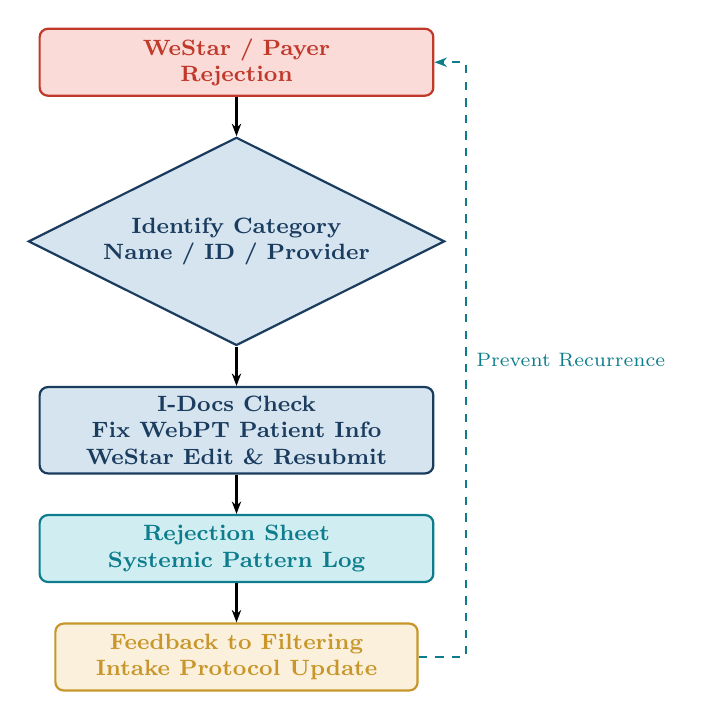
\begin{tikzpicture}[node distance=0.5cm,every node/.style={align=center,font=\scriptsize\bfseries}]
  \node[nR,minimum width=5.0cm] (rej) {WeStar / Payer\\Rejection};
  \node[dB,minimum width=4.6cm,below=0.5cm of rej] (cat) {Identify Category\\Name / ID / Provider};
  \node[nB,minimum width=5.0cm,below=0.5cm of cat] (fix) {I-Docs Check\\Fix WebPT Patient Info\\WeStar Edit \& Resubmit};
  \node[nT,minimum width=5.0cm,below=0.5cm of fix] (sheet) {Rejection Sheet\\Systemic Pattern Log};
  \node[nG,minimum width=4.6cm,below=0.5cm of sheet] (feed) {Feedback to Filtering\\Intake Protocol Update};

  \draw[arr](rej)--(cat);
  \draw[arr](cat)--(fix);
  \draw[arr](fix)--(sheet);
  \draw[arr](sheet)--(feed);
  \draw[arr,dashed,AccentTeal,thick]
    (feed.east)--++(0.6,0)|-(rej.east)
    node[right,font=\scriptsize,pos=0.25]{Prevent Recurrence};
\end{tikzpicture}
\end{center}

\begin{tcolorbox}[infobox,title={Rejection Categories \& Corrective Actions}]
\small
\begin{tabularx}{\linewidth}{L{3.2cm} X L{3.4cm}}
  \rowcolor{TableHead}
  \color{white}\textbf{Category} & \color{white}\textbf{Root Cause} & \color{white}\textbf{Corrective Action} \\
  \textbf{Name Mismatch}
    & Claim name $\neq$ insurance card
    & I-Docs verify; update Patient Info \\
  \rowcolor{TableAlt}
  \textbf{Invalid Member ID}
    & Typo or missing `R' prefix (Medicare)
    & Cross-ref card; fix ID in WebPT \\
  \textbf{Provider Not Found}
    & Provider not credentialed at location
    & Link provider in Billing; resubmit \\
\end{tabularx}
\end{tcolorbox}


%============================================================
\section{Operational Summary and Future Optimization}
%============================================================

The integration of authorization and billing is a continuous loop where accuracy at the point of intake dictates success at the point of submission. Maintaining financial stability requires proactive management of the technical ``Bending'' queue and strict adherence to clinical-billing alignment.

\subsection{Critical Success Factors}

\begin{itemize}
  \item \textbf{Real-Time Data Updates:} Active participation in Cluster Chats to stay ahead of changing payer portal behaviors.
  \item \textbf{Strict BCS Logic Adherence:} Ensuring ``No'' means ``No'' to prevent the delivery of uncompensated care, particularly for MTG and Workers' Comp.
  \item \textbf{Proactive Medicare Cap Tracking:} Calculating the ``Total Spent'' in the portal daily to ensure accurate Kx modifier application.
  \item \textbf{Case ID Integrity:} Ensuring clinical notes are assigned to the correct Case ID (e.g., Lumbar) to prevent diagnostic rejections at the clearinghouse.
\end{itemize}

\vspace{0.4em}
\begin{center}
\textbf{\color{AccentTeal}Diagram I --- Continuous Feedback Loop}\\[0.5em]
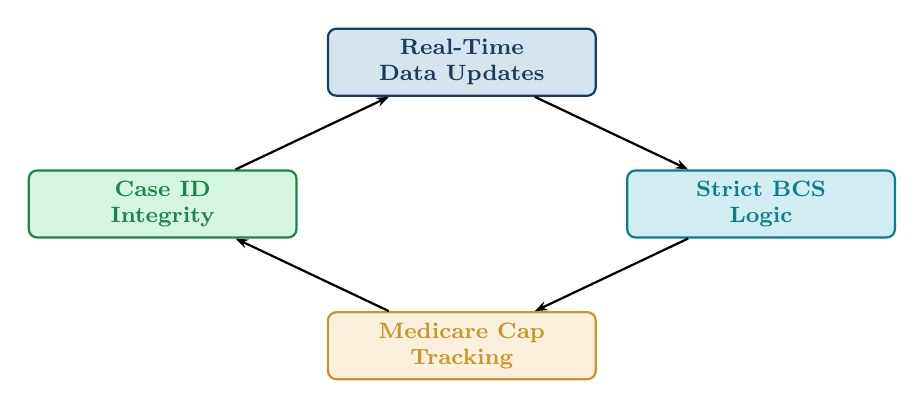
\begin{tikzpicture}[every node/.style={align=center,font=\scriptsize\bfseries}]
  \node[nB,minimum width=3.4cm] (rt) at (0,1.8) {Real-Time\\Data Updates};
  \node[nT,minimum width=3.4cm] (bcs) at (3.8,0) {Strict BCS\\Logic};
  \node[nG,minimum width=3.4cm] (mcap) at (0,-1.8) {Medicare Cap\\Tracking};
  \node[nV,minimum width=3.4cm] (case) at (-3.8,0) {Case ID\\Integrity};

  \draw[arr](rt)--(bcs);
  \draw[arr](bcs)--(mcap);
  \draw[arr](mcap)--(case);
  \draw[arr](case)--(rt);
\end{tikzpicture}
\end{center}

\vspace{0.5em}
\begin{center}
\begin{minipage}[t]{0.47\linewidth}
  \begin{tcolorbox}[metricbox]
    \textbf{\color{AccentTeal}Coverage Control}\\[0.3em]
    BCS audit before every visit. Cluster Chats for live payer updates.
  \end{tcolorbox}
\end{minipage}\hfill
\begin{minipage}[t]{0.47\linewidth}
  \begin{tcolorbox}[metricbox]
    \textbf{\color{AccentTeal}Authorization Control}\\[0.3em]
    Workload secures pre-approvals. Hard stops for W/C and No-Fault.
  \end{tcolorbox}
\end{minipage}\\[0.5em]
\begin{minipage}[t]{0.47\linewidth}
  \begin{tcolorbox}[metricbox]
    \textbf{\color{AccentTeal}Billing Accuracy}\\[0.3em]
    Case ID alignment. Clear billing exceptions before release.
  \end{tcolorbox}
\end{minipage}\hfill
\begin{minipage}[t]{0.47\linewidth}
  \begin{tcolorbox}[metricbox]
    \textbf{\color{AccentTeal}Cash Flow Protection}\\[0.3em]
    Medicare cap checks. Rejection sheet feedback to intake.
  \end{tcolorbox}
\end{minipage}
\end{center}

%============================================================
% CLOSING
%============================================================
\vspace{1.0em}
\begin{tcolorbox}[enhanced,colback=PrimaryBlue,colframe=AccentGold,
    boxrule=2pt,arc=6pt,left=12pt,right=12pt,top=10pt,bottom=10pt]
  \begin{center}
    \color{white}\large\bfseries Core Objective\\[0.5em]
    \color{SoftBlue}\normalsize
    Authorization accuracy at intake, billing integrity at release,\\
    and rejection correction at submission --- together they protect clinic revenue.\\[0.5em]
    \color{AccentGold}\small\textit{Every BCS decision, Bending hold, and Case ID assignment
    has a direct financial consequence.}
  \end{center}
\end{tcolorbox}

\vspace{0.6em}
\begin{center}
  \color{MidGray}\small
  \textit{AI Department --- Prepared by Eng.\ Abdulrahman Hamdi, AI Engineer --- 2026}
\end{center}

\end{document}
